\documentclass{article}
\usepackage[utf8]{inputenc}
\usepackage{amsmath}
\usepackage{amssymb}
\usepackage{graphicx}
\usepackage{subfig}
\usepackage{tcolorbox}
\usepackage{listings}
\usepackage[left=20mm, right=20mm]{geometry}
\usepackage{enumitem}
\usepackage{amsthm}
\usepackage[hyphens]{url}
\usepackage{amsmath}
\usepackage{pgfplots} % Ensure this is included for plots

\newcommand{\Z}{\mathbb{Z}}
\newcommand{\R}{\mathbb{R}}
\renewcommand{\a}{\land}
\renewcommand{\o}{\lor}
\newcommand{\n}{\neg}
\renewcommand{\i}{\implies}
\newcommand{\p}[1]{\begin{pmatrix} #1\end{pmatrix}}
\newtheorem{theorem}{Theorem}
\newtheorem{lemma}[theorem]{Lemma}

\renewcommand\arraystretch{2}

\title{MATH1061 Assignment 2}
\author{SID: 530328265 - Tutorial\_1: 9.00 WED - Tutorial\_2: 10.00 FRI}
\date{Due Date: 12/5/2024}

\begin{document}
	\maketitle
	\section*{1. }
    \begin{figure}[htbp]
        \centering
        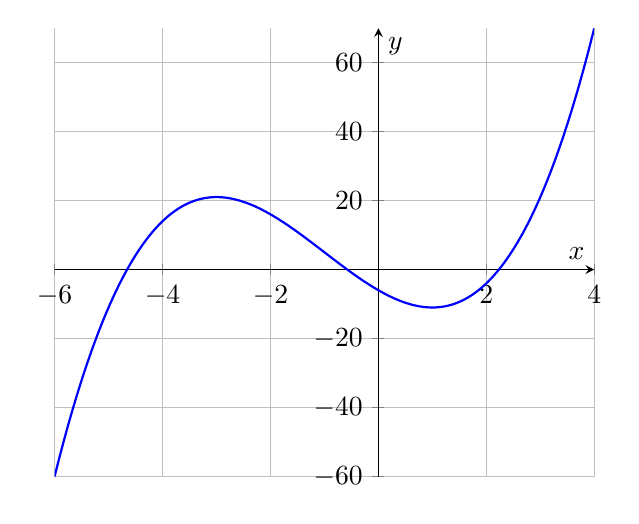
\begin{tikzpicture}
            \begin{axis}[
                axis lines = middle,
                xlabel = \(x\),
                ylabel = {\(y\)},
                grid=major,
                ]
                \addplot[
                    domain=-6:4,
                    samples=100,
                    smooth,
                    thick,
                    blue,
                ]{x^3 + 3*x^2 - 9*x - 6};
            \end{axis}
        \end{tikzpicture}
        \caption{Graph of the function \(y = x^3 + 3x^2 - 9x - 6\)}
    \end{figure}
	\begin{enumerate}[label=({\alph*})]
        \item \textbf{A critical point} of \(f(x)\) is a number \(c\) in the domain of \(f\), where either \(f'(c) = 0\) or where \(f\) is not differentiable at \(c\). To find the critical points for \(f(x) = x^{3} + 3x^{2} - 9x - 6\), we take the first derivative and set it to zero.
        \begin{align}
            f'(x) &= 3x^2 + 6x - 9 = 0 \\
            &= 3(x^2 + 2x - 3) = 0 \\
            &= 3(x^2 + 3x - x - 3) = 0 \\
            &= 3((x^2 + 3x) - (x + 3)) = 0 \\
            &= 3(x(x + 3) - 1(x + 3)) = 0\\
            &= 3(x - 1)(x + 3) = 0 \\
            &= 3(x + 3)(x - 1) = 0\\
        \end{align}
        Thus, \(x = -3\) and \(x = 1\) are the roots of \(f^{'}(x)\). At the same time, both of them on \([-4, 5]\), so \(x = -3\) and \(x = 1\) are the critical points for \(f(x)\) on \([-4, 5]\)

        \textbf{Classifying: Taking the second derivative test}

        We have the first derivatition of \(f(x)\) is \(3x^{2} + 6x - 9\). Thus, second derivatition of \(f(x)\) is:
        \[f^{''}(x) = 6x + 6\]
        
        We have \(f^{''}(-3) = -12 < 0\) and \(f^{''}(1) = 12 >0\), so we have an conclustion that

        There is a local minimum of \(f\) at x = 1 and there is a local maximum of \(f\) at x = -3

        \item From a), we have \(x = -3\) and \(x = 1\) are the critical points for \(f(x)\) on \([-4, 5]\). To find the global maximum and global minimum values, first we find the values of \(f(x)\) critical points on \([-4, 5]\), and we calculate the values of \(f\) at the endpoints of the interval(-4 and 5). After that, we compare all the numbers obtained in the first two steps. The largest of all the values is the \textbf{global maximum} value and the smallest of these values is the \textbf{global minimum} value.
        \begin{itemize}
            \item The value of \(f\) when \(x = -3\) is:
            \[f(-3) = (-3)^{3} + 3 \times (-3)^{2} - 9 \times (-3) - 6 = 21\]
            \item The value of \(f\) when \(x = 1\) is:
            \[f(1) = 1^{3} + 3 \times (1)^{2} - 9 \times (1) - 6 = -11\]
            \item The value of \(f\) when \(x = -4\) is:
            \[f(-4) = (-4)^{3} + 3 \times (-4)^{2} - 9 \times (-4) - 6 = 14\]
            \item The value of \(f\) when \(x = 5\) is:
            \[f(5) = 5^{3} + 3 \times 5^{2} - 9 \times 5 - 6 = 149\]
        \end{itemize}
        As we can see, with \(x = -3\), \(x = 1\), \(x = -4\) and \(x = 5\), the largest value of \(f(x)\) is \(149\) when \(x = 5\) and the smallest value of \(f(x)\) is \(-11\) when \(x = 1\). Thus, the global maximum of \(f(x)\) on \([-4, 5]\) is \(x = 5\), and the global minimum of \(f(x)\) on \([-4, 5]\) is \(x = 1\)
        
        \item A points of inflection is where the function changes its concavity. For example, from concave up to concave down or vice versa. To find the inflection points we do the following steps
        \begin{itemize}
            \item Step 1: Find the second derivative of \(f\)
            \item Step 2: Set the second derivative to zero to find the potenial points of inflection
            \item Step 3: Check the concavity change around that potential points
        \end{itemize}
        \textbf{Step 1:} We have the first derivatition of \(f(x)\) is \(3x^{2} + 6x - 9\). Thus, second derivatition of \(f(x)\) is:
        \[f^{''}(x) = 6x + 6\]
        \textbf{Step 2:} The potenial point of inflection is:
        \[f^{''}(x) = 6x + 6 = 0 \leftrightarrow x = -1\]
        \textbf{Step 3:} To check the concavity change around that potential points, we have the following table to check the concavity change around \(x = -1\):
        \[
        \begin{array}{c|c|c|c}
            x & -\infty & -1 & +\infty \\
            \hline
            y'' & - & 0 & + \\
        \end{array}
        \]
        As we can see, \(f^{''}(x)\) change from negative to positive as x increase through -1, the concavity changes from concave down to concave up. Therefore, \(x = -1\) is a point of inflection. At the same time, \(-1\) in \([-4, 5]\), so \(f(x)\) have a point of iflection on \([-4, 5]\)
    \end{enumerate}
    \newpage
    \section*{2. }
    \begin{figure}[htbp]
        \centering
        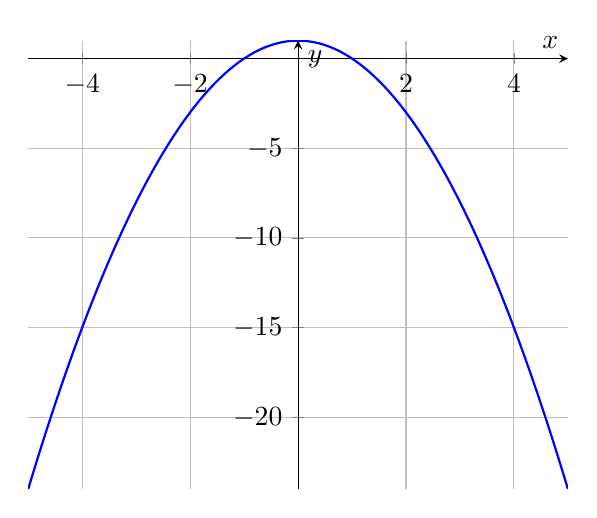
\begin{tikzpicture}
            \begin{axis}[
                axis lines = middle,
                xlabel = \(x\),
                ylabel = {\(y\)},
                grid=major,
                ]
                \addplot[
                    domain=- 5:5,
                    samples=300,
                    smooth,
                    thick,
                    blue,
                ]{1 - x^2};
            \end{axis}
        \end{tikzpicture}
        \caption{Graph of the function \(y = 1 - x^2\)}
    \end{figure}
    \begin{enumerate}[label=({\alph*})]
        \item With integer n \(\leq\) 1, each subinterval has length
        \[\Delta x =  \frac{1 - 0}{n} = \frac{1}{n}\]
        The partion points are given by:
        \[x_{i} = a + \Delta x \times i = 0 + \frac{1}{n} \times i \text{ for }  0 \leq i \leq n\]
        The \(i\)th subinterval will then be the interval \([x_{i - 1}, x_{i}]\)
        \begin{itemize}
            \item Find the lower Riemann sum \(L_{n}\)
            \begin{itemize}
                \item Since \(f(x) = 1 - x^{2}\) is decreasing in \([0, 1]\), the minimum values of \(f(x)\) on any subinterval \([x_{i - 1}, x_{i}]\) occurs at the right endpoint \(x_{i}\). Therefore the lower sum is
                \begin{align}
                    L_{n} &= \sum_{i=1}^n f(x_i) \Delta x = \sum_{i=1}^n \left(1 - \left(\frac{i}{n}\right)^2\right) \frac{1}{n}\\
                          &= \frac{1}{n} \times \sum_{i=1}^n \left(1 - \left(\frac{i}{n}\right)^2\right) \\
                          &= \frac{1}{n} \times  \left(\sum_{i=1}^n(1) - \sum_{i = 1}^n(\frac{i}{n})^2\right)\\
                          &= \frac{1}{n} \times  \left(n - \frac{1}{n^2} \times \sum_{i = 1}^n i^{2}\right) \label{2:a:1}
                \end{align}

                \item We have the following equation:
                \begin{align}
                    \sum_{k=1}^n k^2 = \frac{n(n+ 1)(2n + 1)}{6} \label{2:a:2}
                \end{align}
                \item From \eqref{2:a:1} and \eqref{2:a:2}, we have:
                \begin{align*}
                    L_{n} &= \frac{1}{n} \times \left( n - \frac{1}{n^2} \times \frac{n(n + 1)(2n + 1)}{6}\right) \\
                          &= 1 - \frac{1}{n^{2}} \times \frac{(n + 1)(2n + 1)}{6} \\
                          &= \frac{6n^2 - (n + 1)(2n + 1)}{6n^2} \\
                          &= \frac{6n^2 - (2n^2 + 3n + 1)}{6n^2} \\
                          &= \frac{4n^2 - 3n - 1}{6n^2}
                \end{align*}
            \end{itemize}
            \item Find the upper Riemann sum \(L_{n}\)
            \begin{itemize}
                \item Since \(f(x) = 1 - x^{2}\) is decreasing in \([0, 1]\), the maximum values of \(f(x)\) on any subinterval \([x_{i - 1}, x_{i}]\) occurs at the left endpoint \(x_{i - 1}\). Therefore the lower sum is
                \begin{align}
                    U_{n} &= \sum_{i=1}^n f(x_{i - 1}) \Delta x = \sum_{i=1}^n \left(1 - \left(\frac{i - 1}{n}\right)^2\right) \frac{1}{n}\\
                          &= \frac{1}{n} \times \sum_{i=1}^n \left(1 - \left(\frac{i - 1}{n}\right)^2\right) \\
                          &= \frac{1}{n} \times  \left(\sum_{i=1}^n(1) - \sum_{i = 1}^n(\frac{i - 1}{n})^2\right)\\
                          &= \frac{1}{n} \times  \left(n - \frac{1}{n^2} \times \sum_{i = 1}^n (i - 1)^{2}\right) \\
                          &= \frac{1}{n} \times  \left(n - \frac{1}{n^2} \times \sum_{i - 1 = 0}^{n - 1} (i - 1)^{2}\right) \\
                          &= \frac{1}{n} \times  \left(\left(n - \frac{1}{n^2} \times 0\right) + \left( - \frac{1}{n^2} \times \sum_{i - 1= 1}^{n - 1} (i - 1)^{2}\right)\right) \\
                          &= \frac{1}{n} \times  \left(n + \left( - \frac{1}{n^2} \times \sum_{i - 1= 1}^{n - 1} (i - 1)^{2}\right)\right) \\
                          &= \frac{1}{n} \times  \left(n - \frac{1}{n^2} \times \sum_{i - 1= 1}^{n - 1} (i - 1)^{2}\right) \label{2:a:3}\\
                \end{align}

                \item From \eqref{2:a:3} and \eqref{2:a:2}, we have:
                \begin{align*}
                    U_{n} &= \frac{1}{n} \times \left(n - \frac{1}{n^2} \times \frac{(n - 1)n(2(n - 1) + 1)}{6}\right) \\
                          &= \frac{1}{n} \times \left(n - \frac{1}{n^2} \times \frac{(n - 1)n(2n - 1)}{6}\right) \\
                          &= 1 - \frac{(n - 2)(2n - 1)}{6n^2} \\
                          &= \frac{6n^2 - (n - 1)(2n - 1)}{6n^2} \\
                          &= \frac{6n^2 - (2n^2 - 3n + 1)}{6n^2} \\
                          &= \frac{6n^2 - (2n^2 - 3n + 1)}{6n^2} \\
                          &= \frac{4n^2 + 3n - 1}{6n^2} \\
                \end{align*}
            \end{itemize}
        \end{itemize}
        \item We compute the limit as \(n \to \infty\) of \(L_{n}\) and \(U_{n}\):
        \begin{itemize}
            \item Calculate the limit as \(n \to \infty\) of \(L_{n}\)
            \begin{align}
                \lim_{n \to \infty}(L(n)) &=  \lim_{n \to \infty}\frac{4n^2 - 3n - 1}{6n^2} = \lim_{n \to \infty} \frac{4 - \frac{3}{n} - \frac{1}{n^2}}{6} \\
                                          &= \frac{4 - 0 - 0}{6} = \frac{4}{6} = \frac{2}{3}
            \end{align}
            \item Calculate the limit as \(n \to \infty\) of \(U_{n}\)
            \begin{align}
                \lim_{n \to \infty}(U(n)) &=  \lim_{n \to \infty}\frac{4n^2 + 3n - 1}{6n^2} = \lim_{n \to \infty} \frac{4 + \frac{3}{n} - \frac{1}{n^2}}{6} \\
                                          &= \frac{4 + 0 - 0}{6} = \frac{4}{6} = \frac{2}{3}
            \end{align}
            \item As we can see, \(\lim_{n \to \infty}L(n) = \lim_{n \to \infty}U(n)\) = \(\frac{2}{3}\).
            \item Not only that, \(f(x)\) is decreasing on the interval \([0, 1]\) so we have:
            \[L(n) \leq \int_0^1 (1 - x^2) \, dx \leq U(n)\]
            \item Applying squeeze law, then we have
            \[
                \int_0^1 (1 - x^2) \, dx = \frac{2}{3}
                \]
        \end{itemize}
    \end{enumerate}
    \newpage
    \section*{3. }
    \begin{enumerate}[label=({\alph*})]
        \item First we find the first and second derivative of \(f(x)\):
        \begin{itemize}
            \begin{align*}
                f^{'}(x) &= (2x + 5)e^{-x} - e^{-x}(9 + 5x + x^2) \\
                f^{''}(x) &= 2e^{-x} - (5 + 2x)e^{-x} - (2x + 5)e^{-x} + e^{-x}(9 + 5x + x^2) \\
            \end{align*}
            \item Second, we find the value of \(f^{'}(0) \text{ and } f^{''}(0) \text{ and } f(0)\)
            \begin{align}
                f(0) &= 9 + 5 \times 0 + 0 \times 2 \times e^{-0} = 9 \\
                f^{'}(0) &= (2 \times 0 + 5)e^{-0} + e^{-0}(9 + 5 \times 0 + 0^2) = -4 \\
                f^{''}(0) &=  2e^{-0} - (5 + 2 \times 0)e^{-0} - (2 \times 0 + 5)e^{-0} + e^{-0}(9 + 5 \times 0 + 0^2) = 1
            \end{align}
        \end{itemize}
        From that, we can find \(P_{2}(x)\), which is:
        \begin{align}
            P_{2}(x) &= \frac{f(0)}{0!} + \frac{f^{'}(0) \times x}{1!} + \frac{f^{''}(0) \times x^2}{2!} \\
                    &= 9 - 4x + \frac{x^{2}}{2!}
        \end{align}
        \item The lagrange form of the remainder \(R_{n}(x)\) for Taylor series of order n centered at a is given by:
        \[R_{n}(X) = \frac{f^{n + 1}(c)}{(n + 1)!} \times (x - a)^{n + 1}\]
        We have \(R_{2}(x) = \frac{f^{(3)}(c) \times x^3}{3!}\) for \(0 \leq c \leq 1\)
        \begin{align}
            f^{''}(x) &= 2e^{-x} - (5 + 2x)e^{-x} - (2x + 5)e^{-x} + e^{-x}(9 + 5x + x^2) \\
                      &= e^{-x}\left(2 - (5 + 2x) - (2x + 5) + (9 + 5x + x^2) \right) \\
                      &= e^{-x}\left(2 - 5 - 2x - 2x - 5 + (9 + 5x + x^2) \right) \\
                      &= e^{-x}\left(-4x - 8 + (9 + 5x + x^2) \right) \\
                      &= e^{-x}(x^2 + x + 1)  \label{3:b:1}
        \end{align}
        From \eqref{3:b:1}, we can find the \(f^{(3)}(x)\) and we call \(g(x) = f^{(3)}(x)\)
        \begin{align}
            f^{(3)}(x) &=  (e^{-x}(x^2 + x + 1))^{'} \\
                     &= (2x + 1)e^{-x} - e^{-x}(x^2 + x + 1) \\
                     &= e^{-x}(2x + 1 - x^2 - x - 1) \\
                     &= e^{-x}(-x^2 + x) \\
        \end{align}
        Now, we will find the global maximum values of g(x) on \([0, 1]\)
        
        \textbf{Find critical points} for g(x) on \([0, 1]\)
        \begin{itemize}
            \item The first derivatition of \(g(x)\) is:
            \begin{align*}
                g^{'}(x) &= e^{-x}(-2x + 1) - e^{-x}(-x^{2} + x) \\
                &= -e^{-x} \times 2x + e^{-x} + e^{-x} \times x^{2} - e^{-x} \times x \\
                &= e^{-x} \times x^{2} - 3x \times e^{x} + e^{-x} \\
                &= e^{-x} \times (x^{2} - 3x + 1) 
            \end{align*}
            \item Therefore the critical points of \(g(x)\) are the roots of \(g^{'}(x)\):
            \begin{align*}
                e^{-x} \times (x^{2} - 3x + 1) = 0 \\
            \end{align*}
            \item Because \(e^{-x}\) always larger than 0 for all \(x \in \mathbb{R}\). Thus the roots of \(x^{2} - 3x + 1\) are also the root of \(g^{'}(x)\)
            \begin{align}
                &\Delta = \sqrt{(-3)^{2} - 4 \times 1 \times 1} = \sqrt{5} \\
                \rightarrow& x_{1, 2} = \frac{-(-3) \pm \sqrt{5}}{2} 
            \end{align}
            \item Thus, \(x = \frac{3 - \sqrt{5}}{2}\)is the critical points for \(g(x)\) on \([0, 1]\).
            \item The global minimum of \(g(x)\) on \([0, 1]\) is:
            \begin{itemize}
                \item The value of \(g\) when x = 0 is \(g(0) = 0\)
                \item The value of \(g\) when x = \(\frac{3 - \sqrt{5}}{2}\) is \(g(\frac{3 - \sqrt{5}}{2}) \approx 0.16112\)
                \item The value of \(g\) when x = 1 is \(g(1) = 0\)
            \end{itemize}
            \item Thus, the global maximum of \(g\) is \(\approx 0.360\) when x = \(\frac{3 - \sqrt{5}}{2}\)
        \end{itemize}
        We have:
        \[f^{(3)}(c) = (-c^{2} + c)e^{-c} \leq (-1^2 + 1) e^{-1}\]
        Thus,
        \[f^{(3)}(c) \leq 0\]
        At the same time,
        \[R_{2}(x) = \frac{f^{(3)}(c) \times x^{(3)}}{3!} = \frac{g(c) \times x^{(3)    }}{3!} \leq \frac{0.16112 \times x^{3}}{3!}\]
        With \(x = 1\), we have 
        \[R_{2}(1) \leq \frac{0.16112 \times 1^3}{3!} \approx 0.02685\]
        Thus, the upperbound is \(0.02685\)
    \end{enumerate}
    \newpage
    \section*{4. }
        Let \(\ell_1\) and \(\ell_2\) be two lines in space defined by the parametric equations:
        \[
        \ell_1 : \begin{cases}
        x = 3 - s \\
        y = 4 + 5s \\
        z = 3 + s 
        \end{cases}
        \quad (s \in \mathbb{R})
        \]
        \[
        \ell_2 : \begin{cases}
        x = 2 + t \\
        y = -3 + t \\
        z = -2 + 2t
        \end{cases}
        \quad (t \in \mathbb{R})
        \]

        \subsection*{(a)}
        To find the point of intersection, equate the parametric equations:
        \begin{align*}
        3 - s &= 2 + t \\
        4 + 5s &= -3 + t \\
        3 + s &= -2 + 2t 
        \end{align*}
        Solving the system:
        \begin{align*}
            s + t &= 1 \quad \text{(from x-coordinates)} \\
            5s - t &= -7 \quad \text{(from y-coordinates)} \\
            s - 2t &= -5 \quad \text{(from z-coordinates)}
        \end{align*}

        From x\-coordinates and y\-coordinates, we find \(s = -1\) and \(t = 2\). Thus, we plugging back to z\-coordinates to check that s and t is the valid solution or not.
        \[s - 2t = -1 - 2\times 2 = -5 \text{  (VALID SOLUTION)}\]

        We find \(s = -1\) and \(t = 2\). Plugging these back into the line equations gives:
        \begin{align}
            &x = 3 - s = 3 + 1 = 4 \\
            &y = 4 + 5 \times (-1) = -1 \\
            &z = 3 + s = 3 - 1 = 2 \\
        \end{align}
        \[
        \text{Intersection Point: } (4, -1, 2)
        \]

        \subsection*{(b)}
        To find a general equation for the plane \(P\) that contains both \(\ell_1\) and \(\ell_2\), use the direction vectors of the lines \(\vec{d}_1 = (-1, 5, 1)\) and \(\vec{d}_2 = (1, 1, 2)\) and a point on the plane. The cross product of \(\vec{d}_1\) and \(\vec{d}_2\) gives a normal vector \(\vec{n}\) to the plane:
        \begin{align}
            \vec{n} &= \vec{d}_1 \times \vec{d}_2 = \begin{vmatrix}
                -1 & 5 & 1 \\
                1 & 1 & 2 
                \end{vmatrix} \\
                &= \left((5 \times 2 - 1 \times 1), (1 \times 1 - (-1 \times 2)), (1 \times -1 - 5 \times 1)\right) \\
                &= (9, 3, -6) \\
                &= (3, 1, -2)
        \end{align}
        The normal vector simplifies to \(\vec{n} = (3, 1, -2)\). Using the point of intersection (4, -1, 2), the plane equation is:
        \[
        3(x - 4) + 1(y + 1) - 2(z - 2) = 0
        \]
        This simplifies to:
        \[
        3x - 12 + y + 1 - 2z + 4 = 0
        \]
        Thus, the general equation for plane \(P\) is:
        \[
        3x + y - 2z = 7
        \]
        \newpage
        \section*{5.}
        We start with the augmented matrix of the system:
        \[
        \begin{bmatrix}
        1 & 0 & -5 & | & -4 \\
        1 & -\lambda & -2 & | & 2 \\
        1 & 2 & \lambda & | & 2
        \end{bmatrix}.
        \]
        The goal is to use elementary row operations to transform this matrix into row echelon form. We will perform the following steps:
        
        \textbf{Step 1: Eliminate \(x\) from the second and third rows.}
        \begin{itemize}
            \item \(R_2 \leftarrow R_2 - R_1\): Subtract the first row from the second row.
            \item \(R_3 \leftarrow R_3 - R_1\): Subtract the first row from the third row.
        \end{itemize}
        This results in:
        \[
        \begin{bmatrix}
        1 & 0 & -5 & | & -4 \\
        0 & -\lambda & 3 & | & 6 \\
        0 & 2 & \lambda + 5 & | & 6
        \end{bmatrix}.
        \]
        Then, we take \(R_{3} \leftarrow R_{3} / 2\), after that we swap \(R_{3}\) with \(R_2\)
        \[
        \begin{bmatrix}
        1 & 0 & -5 & | & -4 \\
        0 & 1 & \frac{\lambda + 5}{2} & | & 3 \\
        0 & -\lambda & 3 & | & 6 
        \end{bmatrix}.
        \]
        We take \(R_3 \leftarrow \lambda R_{2} + R_{3}\). Then we will have the row echelon form.
        \[
        \begin{bmatrix}
        1 & 0 & -5 & | & -4 \\
        0 & 1 & \frac{\lambda + 5}{2} & | & 3 \\
        0 & 0 & \frac{\lambda^{2} + 5\lambda + 6}{2} & | &3 \lambda +  6 
        \end{bmatrix}.
        \]
        \textbf{b)} For \(\frac{\lambda^2 + 5 \lambda + 6}{2}z = 6 + 3 \lambda\)
        \begin{itemize}
            \item To make the system has no solution, we have the following equations
            \begin{itemize}
                \item We have
                \begin{align}
                    \frac{\lambda^2 + 5 \lambda + 6}{2}z &= 6 + 3 \lambda \\
                    (\lambda + 2)(\lambda + 3)z &= 12 + 6\lambda \\
                    (\lambda + 2)(\lambda + 3)z &= 6(\lambda + 2)
                \end{align}
                \item To make the system has no solution, we need to make z not exists, which means \(\lambda = -3\) and \(\lambda \neq -2\)(because at this situation (\(0z = -6\)))
                \item Thus the system has no solution if and only if \(\lambda = -3\)
            \end{itemize}
            \item To make the system has infinite solutions, we need to make the equation \((\lambda + 2)(\lambda + 3)z = 6(\lambda + 2)\) always True. Thus, \(\lambda\) equals to \(-2\). The reason for that is when \(\lambda = -2\), we have:
            \begin{itemize}
                \item \begin{equation}
                    0z = 0 \text{    (This one always True)}
                \end{equation}
            \end{itemize}
            \item To make the system has an unique solution, \(\lambda \neq -3\) and \(\lambda \neq -2\). At that time, we have the value of z is \(\frac{6\lambda + 12}{\lambda^{2} + 5 \lambda + 6}\)
        \end{itemize}
        
            
        \newpage
        \section*{6}
        \begin{enumerate}[label = ({\alph*})]
            \item We hav the following transition probalities
            \begin{itemize}
                \item From state 1 (linear algebra)
                \begin{enumerate}
                    \item Stay in State 1: 80\% \((P_{1,1} = 0.8)\)
                    \item Move to State 2 (Calculus): 10\% \((P_{2, 1} = 0.1)\)
                    \item Move to State 3 (Netflix): 10\% \((P_{3, 1} = 0.1)\)
                \end{enumerate}
                \item From State 2(Calculus)
                \begin{itemize}
                    \item Move to State 1: 20\% \((P_{1, 2} = 0.2)\)
                    \item Stay in State 2: 60\% \((P_{2, 2} = 0.6)\)
                    \item Move to State 3: 20\% \((P_{3, 2} = 0.2)\)
                \end{itemize}
                \item From State 3(Netflix)
                \begin{itemize}
                    \item Move to State 1: 40\% \((P_{1, 3} = 0.4)\)
                    \item Stay to State 2: 40\% \((P_{2, 3} = 0.4)\)
                    \item Stay in State 3: 20\% \((P_{3, 3} = 0.2)\)
                \end{itemize}
                \item Hence, we have the following matrix
                \[P = \begin{bmatrix}
                    0.8 & 0.2 & 0.4 \\
                    0.1 & 0.6 & 0.4 \\
                    0.1 & 0.2 & 0.2 \\
                \end{bmatrix}
                \]
            \end{itemize}
                \item we have:
                \begin{itemize}
                \item \[\vec{x_{0}} = 
                \begin{bmatrix}
                    1000 \\
                    1000 \\
                    800 \\
                \end{bmatrix}
                    \]
                \item Let \(x_{2}\) is the number of each state on day 2. Thus, \(x_{2}\) equals to:
                \[\vec{x_{2}} = P \times \vec{x_{1}} = P \times P \times \vec{x_{0}} = P^{2} \times \vec{x_{0}}\]
                \item Calculate \(P^{2}\)
                \begin{align}
                    P^2 &= \begin{bmatrix}
                        0.8 & 0.2 & 0.4 \\
                        0.1 & 0.6 & 0.4 \\
                        0.1 & 0.2 & 0.2
                        \end{bmatrix}
                        \cdot
                        \begin{bmatrix}
                        0.8 & 0.2 & 0.4 \\
                        0.1 & 0.6 & 0.4 \\
                        0.1 & 0.2 & 0.2
                        \end{bmatrix} \\
                    &= \begin{bmatrix}
                        (0.8\cdot0.8 + 0.2\cdot0.1 + 0.4\cdot0.1) & (0.8\cdot0.2 + 0.2\cdot0.6 + 0.4\cdot0.2) & (0.8\cdot0.4 + 0.2\cdot0.4 + 0.4\cdot0.2) \\
                        (0.1\cdot0.8 + 0.6\cdot0.1 + 0.4\cdot0.1) & (0.1\cdot0.2 + 0.6\cdot0.6 + 0.4\cdot0.2) & (0.1\cdot0.4 + 0.6\cdot0.4 + 0.4\cdot0.2) \\
                        (0.1\cdot0.8 + 0.2\cdot0.1 + 0.2\cdot0.1) & (0.1\cdot0.2 + 0.2\cdot0.6 + 0.2\cdot0.2) & (0.1\cdot0.4 + 0.2\cdot0.4 + 0.2\cdot0.2)
                        \end{bmatrix}\\
                    &= \begin{bmatrix}
                    0.7 & 0.36 & 0.48 \\
                    0.18 & 0.46 & 0.36 \\
                    0.12 & 0.18 & 0.16
                    \end{bmatrix}
                    \end{align}
                    \item Therefore, \(\vec{x_2}\) is calculated as follows:
                    \begin{align*}
                    \vec{x_2} &= P^2 \cdot \vec{x_0} \\
                        &= \begin{bmatrix}
                            0.7 & 0.36 & 0.48 \\
                            0.18 & 0.46 & 0.36 \\
                            0.12 & 0.18 & 0.16
                        \end{bmatrix}
                        \cdot
                        \begin{bmatrix}
                            1000 \\
                            1000 \\
                            800
                        \end{bmatrix} \\
                        &= \begin{bmatrix}
                            (0.7 \cdot 1000 + 0.36 \cdot 1000 + 0.48 \cdot 800) \\
                            (0.18 \cdot 1000 + 0.46 \cdot 1000 + 0.36 \cdot 800) \\
                            (0.12 \cdot 1000 + 0.18 \cdot 1000 + 0.16 \cdot 800)
                        \end{bmatrix} \\
                        &= \begin{bmatrix}
                            700 + 360 + 384 \\
                            180 + 460 + 288 \\
                            120 + 180 + 128
                        \end{bmatrix} \\
                        &= \begin{bmatrix}
                            1444 \\
                            928 \\
                            428
                        \end{bmatrix}
                    \end{align*}
                    \item Thus, there are
                    \begin{itemize}
                        \item 1444 students in state 1
                        \item 928 students in state 2
                        \item 428 students in state 3
                    \end{itemize}
            \end{itemize}
            \item Expanding \((P - I_{3})\vec{x} = 0\), we have:
            \begin{align*}
                (P - I_3)\vec{x} &= 0 \\
                Px - I_{3}\vec{x} &= 0 \\
            \end{align*}
            Since \(I_{3}\vec{x} = \vec{x}\)(identity matrix leaves vectors unchanged), the equation simplifies to \(Px = x\)

            Let \(\vec{x} = \begin{bmatrix} x \\ y \\ z \end{bmatrix}\). We have:
            \begin{align*}
                P\vec{x} &= \vec{x} \\
                \begin{bmatrix}
                    0.8 & 0.2 & 0.4 \\
                    0.1 & 0.6 & 0.4 \\
                    0.1 & 0.2 & 0.2
                \end{bmatrix}
                \cdot
                \begin{bmatrix}
                    x \\
                    y \\
                    z
                \end{bmatrix}
                &= 
                \begin{bmatrix}
                    x \\
                    y \\
                    z
                \end{bmatrix}\\
            \end{align*}
            Then, we have the equations
            \begin{align*}
                0.8x + 0.2y + 0.4z &= x \\
                0.1x + 0.6y + 0.4z &= y \\
                0.1x + 0.2y + 0.2z &= z
            \end{align*}
            Which equals to:
            \begin{align*}
                -0.2x + 0.2y + 0.4z &= 0 \\
                0.1x - 0.4y + 0.4z &= 0 \\
                0.1x + 0.2y - 0.8z &= 0
            \end{align*}
            From that equations, we have the an augmented matrix:
            \[
            \begin{bmatrix}
            -0.2 & 0.2 & 0.4 & | & 0 \\
            0.1 & -0.4 & 0.4 & | & 0 \\
            0.1 & 0.2 & -0.8 & | & 0
            \end{bmatrix}.
            \]
            First, we take \(R_{1} \leftarrow R_{1}/-2\) and \(R_{2} \leftarrow R_{2} - R_{3}\), then we have
            \[
            \begin{bmatrix}
            0.1 & -0.1 & -0.2 & | & 0 \\
            0 & -0.6 & 1.2 & | & 0 \\
            0.1 & 0.2 & -0.8 & | & 0
            \end{bmatrix}.
            \]
            Then, we take \(R_{2} \leftarrow \frac{R_{2}}{2}\) and \(R_{3} \leftarrow R_{3} - R_{1}\)
            \[
            \begin{bmatrix}
            0.1 & -0.1 & -0.2 & | & 0 \\
            0 & -0.3 & 0.6 & | & 0 \\
            0 & 0.3 & -0.6 & | & 0
            \end{bmatrix}.
            \]
            Finally, we take \(R_{3} \leftarrow R_{3} + R_{2}\)
            \[
            \begin{bmatrix}
                0.1 & -0.1 & -0.2 & | & 0 \\
                0 & -0.3 & 0.6 & | & 0 \\
                0 & 0 & 0 & | & 0
                \end{bmatrix}.
                \]
            As we can see \(R_{3}\) has infinite solutions, since 0 always = 0(z can be anything)

            Hence we have infinite solution for \(\vec{x}\)

            We have equations that:
            \[x - y - 2z = 0\]
            \[y - 2z = 0\]

            Let \(z = t\), then  \(x = 3t\) and \(y = 2t\)

            Thus, we got vector x:
            \[\vec{x} = \begin{bmatrix}
                4t \\
                2t \\
                t
            \end{bmatrix}\]
        \item We have:
        \[x_{0} = \begin{bmatrix}
            1600\\
            800\\
            400
        \end{bmatrix} = \begin{bmatrix}
            4 \times 400 \\
            2 \times 400 \\
            400
        \end{bmatrix} = \begin{bmatrix}
            4t \\
            2t \\
            t
        \end{bmatrix} (\text{With t = 400})\]

        Because we have x has the form in question c, we have the properties that have been proved in 6b, which is:
        \[Px = x\]
        
        We have \(x_{1} = Px_{0} = x_{0}\), which implies to:

        \[x_{100} = Px_{99} = P(Px_98) = P(P(Px_{97})) = P(P(P...(Px_0)))(\text{We will have } 100P_{s})\]

        Thus, \(x_{100}\) equals to:
        \[x_{100} = \begin{bmatrix}
            1600 \\
            800 \\
            400 
        \end{bmatrix}\]
    \end{enumerate}
\end{document}
